% hubbletilus_annotated.tex -- Hubble corner plot styled to match
% pearltilus_annotated.tex. All five parameters (sdx sdy sdz stx sty) belong
% to the secondary mirror. Overlays ../figures/hubbletilus.png (panels: 200 px
% squares on a 210 px pitch, first panel at x=84, y=36 px).
% The small corner titles and tick labels are covered and replaced by large
% parameter names and a summary table. Table values are the full-posterior
% medians and 16-84% intervals printed in the original corner titles
% (translations rounded to 1 um); axis spans are read from the tick marks.
% Build: pdflatex hubbletilus_annotated.tex
\documentclass[tikz,border=4pt]{standalone}
\usepackage[T1]{fontenc}
\usepackage[default]{sourcesanspro}
\usepackage{booktabs}
\usetikzlibrary{calc}
\definecolor{sec}{HTML}{F58518}
\newlength\pxu
\setlength\pxu{0.026203cm}   % 1143 px -> 29.95 cm
\begin{document}
\begin{tikzpicture}[x=\pxu, y=\pxu]
  \node[anchor=south west, inner sep=0pt] at (0,0)
    {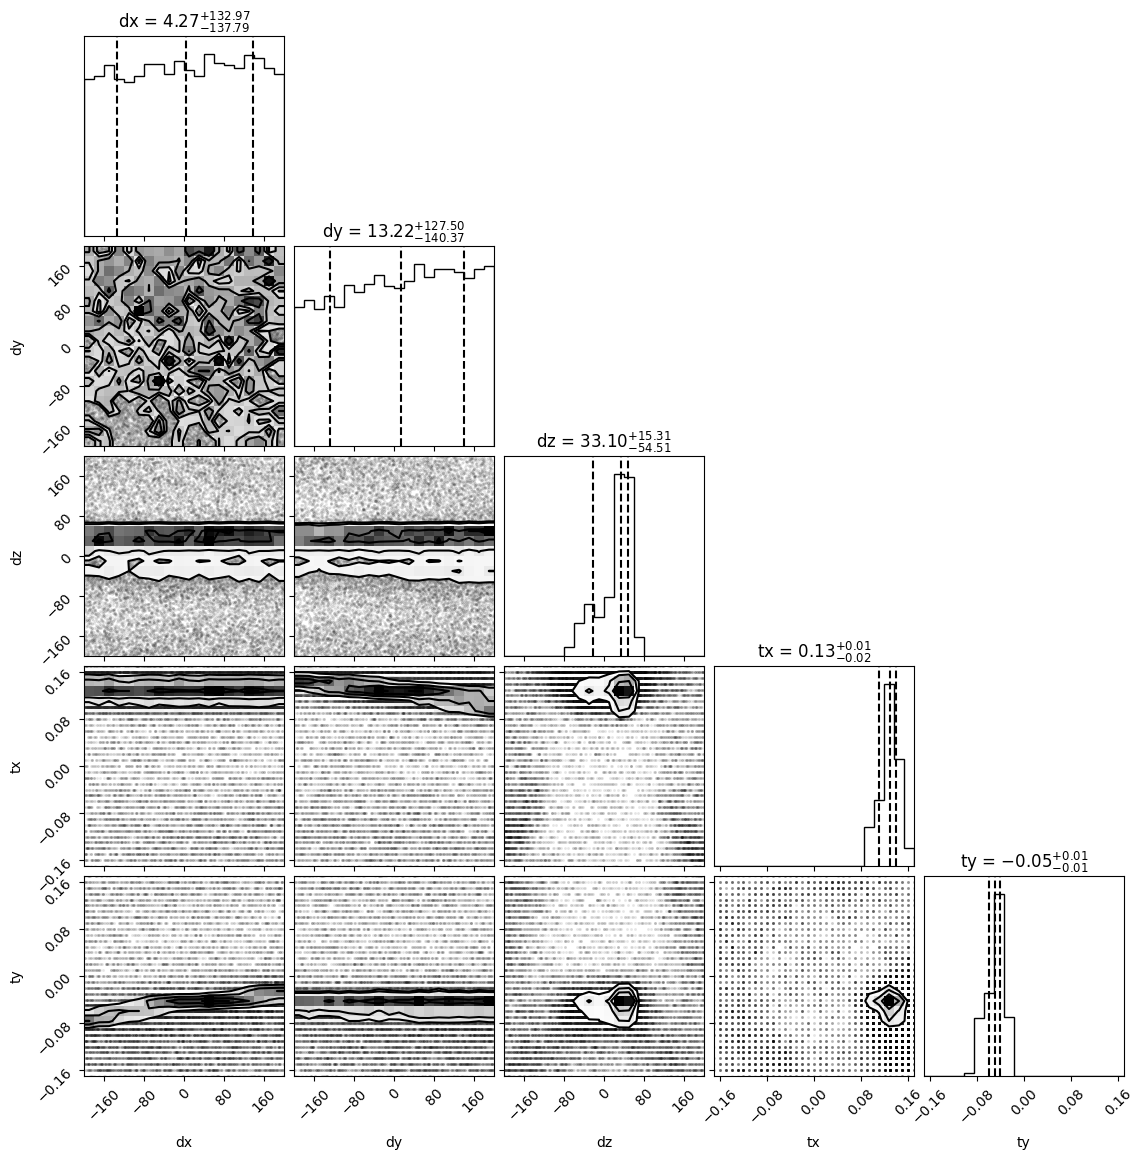
\includegraphics[width=1143\pxu]{../figures/hubbletilus.png}};
  % Tint every panel: all pairs are secondary-mirror pairs.
  \begin{scope}[blend mode=multiply]
    \fill[sec!12] (84,924) rectangle (284,1124);
    \fill[sec!12] (84,714) rectangle (284,914);
    \fill[sec!12] (294,714) rectangle (494,914);
    \fill[sec!12] (84,504) rectangle (284,704);
    \fill[sec!12] (294,504) rectangle (494,704);
    \fill[sec!12] (504,504) rectangle (704,704);
    \fill[sec!12] (84,294) rectangle (284,494);
    \fill[sec!12] (294,294) rectangle (494,494);
    \fill[sec!12] (504,294) rectangle (704,494);
    \fill[sec!12] (714,294) rectangle (914,494);
    \fill[sec!12] (84,84) rectangle (284,284);
    \fill[sec!12] (294,84) rectangle (494,284);
    \fill[sec!12] (504,84) rectangle (704,284);
    \fill[sec!12] (714,84) rectangle (914,284);
    \fill[sec!12] (924,84) rectangle (1124,284);
  \end{scope}
  % Cover the small titles and tick labels (tick marks are kept)
  \fill[white] (84,1127) rectangle (284,1160);
  \fill[white] (294,917) rectangle (494,958);
  \fill[white] (504,707) rectangle (704,748);
  \fill[white] (714,497) rectangle (914,538);
  \fill[white] (924,287) rectangle (1124,328);
  \fill[white] (0,0) rectangle (1143,75);
  \fill[white] (0,75) rectangle (74,914);
  % Large parameter names
  \node[font=\fontsize{26}{30}\selectfont] at (184.0,37.5) {$sdx$};
  \node[font=\fontsize{26}{30}\selectfont] at (394.0,37.5) {$sdy$};
  \node[font=\fontsize{26}{30}\selectfont] at (604.0,37.5) {$sdz$};
  \node[font=\fontsize{26}{30}\selectfont] at (814.0,37.5) {$stx$};
  \node[font=\fontsize{26}{30}\selectfont] at (1024.0,37.5) {$sty$};
  \node[rotate=90, font=\fontsize{26}{30}\selectfont] at (37,814.0) {$sdy$};
  \node[rotate=90, font=\fontsize{26}{30}\selectfont] at (37,604.0) {$sdz$};
  \node[rotate=90, font=\fontsize{26}{30}\selectfont] at (37,394.0) {$stx$};
  \node[rotate=90, font=\fontsize{26}{30}\selectfont] at (37,184.0) {$sty$};
  % Mirror group along the columns (x axis)
  \fill[sec] (84,-49.6) rectangle (1124,-7.6);
  \node[text=white, font=\bfseries\fontsize{20}{24}\selectfont] at (604.0,-28.6) {SECONDARY};
  % Summary table in the empty upper-right triangle
  \node[anchor=north east, inner sep=0pt] (tab) at (1114,1110) {%
    \fontsize{24}{34}\selectfont
    \begin{tabular}{@{}lrll@{}}
      \toprule
      & \bfseries Median & \bfseries 68\% & \bfseries Axis span \\
      \midrule
      \textcolor{sec!85!black}{\bfseries $sdx$} & $4$ & $^{+133}_{-138}$ & $\pm200\,\mu$m \\
      \textcolor{sec!85!black}{\bfseries $sdy$} & $13$ & $^{+128}_{-140}$ & $\pm200\,\mu$m \\
      \textcolor{sec!85!black}{\bfseries $sdz$} & $33$ & $^{+15}_{-55}$ & $\pm200\,\mu$m \\[3pt]
      \textcolor{sec!85!black}{\bfseries $stx$} & $0.13$ & $^{+0.01}_{-0.02}$ & $\pm0.17^{\circ}$ \\
      \textcolor{sec!85!black}{\bfseries $sty$} & $-0.05$ & $\pm0.01$ & $\pm0.17^{\circ}$ \\
      \bottomrule
    \end{tabular}};
  % Legend below the table
  \node[anchor=north east, align=left, font=\fontsize{20}{30}\selectfont,
        fill=white, draw=black!25, inner sep=12pt] at ($(tab.south east)+(0,-20)$) {%
    \textcolor{sec!25}{\rule{1.1em}{0.8em}}\ Secondary-mirror pair};
\end{tikzpicture}
\end{document}
